%
%	Begrifflichkeiten
%

\pagebreak
\section{Targeting}

\onehalfspacing

\subsection{Targeted Advertising}

\subsubsection{Rationale}

Why do we need targeted advertising?

Let's start with the basics: Any advertising or marketing business has a vested interest to make their ads relevant, especially on the world wide web, where the user is, at least to a certain extent, anonymous. In its very basic, offline form, agencies would use context to place their ads; as an example, we might see advertising for cars on busy roads or advertising for food near supermarkets.

In the online world, targeting users can be much more granular and automated, with the ideal outcome of showing an ad exactly at the right time and the right place (e.g., web site) for the user to see it, and with a need that it fulfills, have the user buy the product.

Showing personalized advertisement by targeting the right user at the right time is essential for established as well as new market entrants.

In a recent report, \href{https://www2.deloitte.com/de/de.html}{Deloitte} found that 74\% of small businesses using personalized ads stated that they were important for the success of their business.\footnote{See \textit{Deloitte LLP (2021)}: Dynamic Markets \cite{deloitteSmb}} 68\% of the surveyed small companies said that the use of personalized, targeted advertising helped them to achieve a higher return on their marketing spend.

To achieve this and show personalized and targeted advertising, ad placement uses micro-targeting on the world wide web.

"Microtargeting is a marketing strategy that uses people’s data — about what they like, who they’re connected to, what their demographics are, what they’ve purchased, and more — to segment them into small groups for content targeting. It’s the reason that if you typically shop at Whole Foods, you may be served an advertisement for organic sunscreen during the Summer. And while it can help deliver content that is interesting and helpful to you, it also has a dark side — especially if it delivers information that’s inaccurate or biased and meant to sway your vote."\footnote{\textit{Ghosh, D. (2018)}: What is microtargeting? \cite{mozillaBlog}}

From a business point of view, showing personalized ads through micro-targeting dramatically increases the relevance of the displayed advertising and thus the likelihood of the user noticing it. Even if it does not lead to a sale right away, any product awareness helps and might lead to a deal in the future. 

Give the automated nature of ad placement on web pages, there is no longer a need for ads to be shown in bulk, like in the offline world, but can be displayed individually and with high relevance. 

\subsubsection{Tracking}

To achieve this, it is necessary to gather more information on a particular user's interests and follow their interests across the web; this mechanism is called tracking. Tracking as of today heavily relies on the use of cookies, small pieces of information stored in the users' browser, which we will explain in the next section.

Tracking can span web sites and companies - it is not limited to one company keeping a record of one's visits; currently it also includes the ability to analyze all visits on cooperating pages and show, for example, ads on Facebook based on our recent queries at Amazon. Technically this can be achieved through third-party cookies.

Third-party cookies are cookies set by another website other than the one we're currently visiting, which can be later evaluated from any website.\footnote{See \textit{Cookie Script (2021)}: All you need to know about Third-Party Cookies \cite{mozillaBlog}}

Tracking through third-party cookies is under attack from multiple angles;\footnote{See \textit{Brinkmann, M. (2021)}: How Firefox new SmartBlock feature works \cite{mozillaBlog}} even \href{https://www.google.com/}{Google}, who invented it among various other tracking methods, will no longer support it in \href{https://www.google.com/chrome/}{Chrome} after 2023.\footnote{See \textit{Goel, V. (2021)}: An updated timeline for Privacy Sandbox milestones. \cite{sandboxDelay}}

Placing targeted ads currently makes heavy use of tracking, especially in the form of tracking cookies; however, it can also make use of publicly available information, such as social media posts, as we will see later in this paper.

\subsubsection{Cookies}

Let's go back to cookies and have a look at what it is.

A cookie is a small piece of information that a server sends to the user's web browser for storage and which it can request back at a later point in time.

Cookies can be used for session management, personalizing and tracking.\footnote{See \textit{Mozilla (2021)}: Using HTTP cookies \cite{usingCookies}} For the purpose of this paper, we will focus solely on the tracking aspect, especially across sites, and do not cover the more benign use cases for cookies, such as session management, in any detail.

This explanation shows that cookies themselves are not malign and significantly support the user's experience across the web. However, they also include a persistent history of the user's activities, which can track the users' journey across the web.

Let's have a look at where cookies live on a user's browser. As an example, we will look at \href{https://www.mozilla.org/en-US/firefox/new/}{Firefox}, which stores its cookies in a \href{https://www.sqlite.org/index.html}{SQLite} database in the user's profile directory. Here's a screenshot using \href{https://sqlitebrowser.org/}{DB Browser for SQLite} to have a look at the cookies on our computer:

\begin{figure}[H]
\centering
\caption{Screenshot - Cookie Details in Firefox}
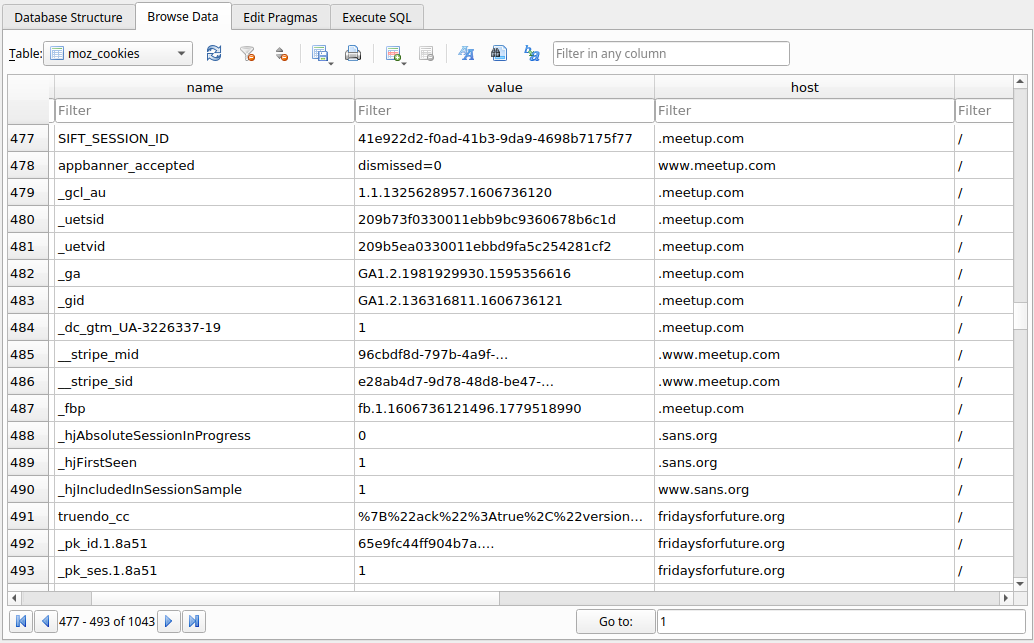
\includegraphics[width=\linewidth]{images/cookie-sqlite.png}
\label{fig:cookies}
\end{figure}

In its technical essence, cookies are a simple key-value store in the browser that stores the data per host, or more precisely, per web site. It's entirely up to the web site to define which keys it wants to store and which values it wants to set and thus persist across visits. 

If a web site accesses its own cookies (as defined in the hosts column), that's called accessing first party cookies and it's part of first party data. For example, this could be used for session persistence, as seen in the first row of the image above. 

If a web site accesses data from another site, that's when we're talking about referencing third party cookies as part of third-party data. Data from other web site's cookies could be used to track users on their visits across different web sites and has become a big privacy concern over the last couple of years. This tracking aspect across sites is what primarily motivates this paper.

We will define the various data types in the next chapter.

In addition to tracking in the web browser, there's also tracking in E-Mail, however, we will not cover E-Mail tracking in this paper.\footnote{See \textit{Doffmann, Z. (2021)}: Why You Suddenly Need To Delete Gmail On Your iPhone \cite{deleteGmail}}

\subsection{Data Types}

\subsubsection{First Party}

Now that we have covered cookies as a mechanism to persist data in the user's browser across sessions, we need to look at the various classes of data, define their usage and prepare for the analysis of their relevance regarding to privacy regulations.

The definition for first party data is actually quite simple; it is data that we collect from our own sources.\footnote{See \textit{OnAudience (2019)}: What is first party data? \cite{firstParty}} Data could include information that we retrieve from our own cookies or from any information the user might have left on our website, for example, by looking at an item. It also includes registration information, shop logins, and past sales or other interaction. Collection of this kind of data is not a big issue from a privacy point of view, as long as it's done correctly and with the necessary precautions against abuse in place.

As an example, in a web shop, a clever use case for using one's own shop data for marketing would be to follow up on an abandoned sale. Here's a screenshot on a follow-up E-Mail where the user looked at an item but did not put it into their shopping cart:

\begin{figure}[H]
\centering
\caption {Screenshot - Zumiez Follow-Up E-Mail}
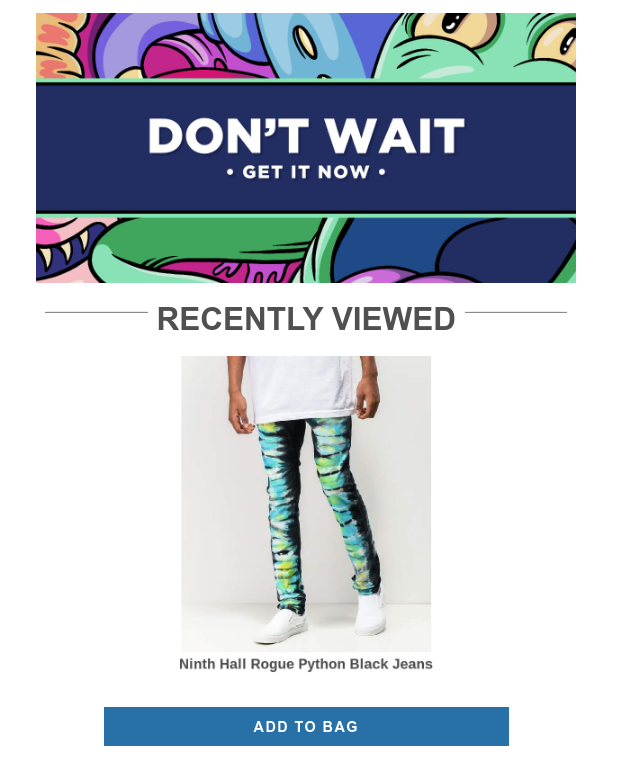
\includegraphics[scale=0.6]{images/zumiez-dont-wait.png}
\label{fig:zumiez}
\end{figure}

This screenshot was taken from an E-Mail by \href{https://www.zumiez.com/}{Zumiez}, prompting the user to follow through with buying an item that they looked at the day before.

Another example of clever use of first-party data for marketing are the advertising \mbox{\href{https://smile.amazon.de/}{Amazon}} places on its own web pages, as we will see further below, or the regular follow-up E-Mails from \href{https://www.netflix.com/de-en/}{Netflix} to finish the season of a series we just started, as shown in the next screenshot:

\begin{figure}[H]
\centering
\caption {Screenshot - Netflix Follow-Up E-Mail (Boruto)}

\includegraphics[scale=0.6]{images/continue-boruto.png}
\label{fig:boruto}
\end{figure}

\subsubsection{Second Party}

The next class of data that we will look at is second party data. Simply speaking, second party data is another companies first party data.\footnote{See \textit{OnAudience (2019)}: What is first party data? \cite{firstParty}}

Assuming that two companies use the same identifier for their customers, for example, the E-Mail address, one company could sell the shopping history on their site to another company to enable them to advertise related products. Another option would be not to sell the data outright but to establish cooperation and use the data from both parties across both web sites.

As we will see later in this paper, from a legal perspective, this is the most challenging setup to achieve. Both companies would need explicit consent from all their users to transfer their data to the other company; they would otherwise open themselves up for a lot of legal trouble and violate the trust and privacy of their customers.

It can be achieved, though, for example, within a conglomerate such as \href{https://www.facebook.com/}{Facebook}, \href{https://www.whatsapp.com/}{WhatsApp} and \href{https://www.instagram.com/}{Instagram}, where platform users are explicitly asked to allow their data to be shared across all platforms. In the case of WhatsApp, the announcement to cooperate on user profiles with the parent company in the short term led to the departure of some users that greatly benefited the competing platforms. In the long term, however, the integration did go well, and the users now experience streamlined profile management and smooth interoperability. Monthly WhatsApp users in July of this year now exceed 2 billion, and their numbers are growing steadily.\footnote{See \textit{Statista (2021)}: Most popular global mobile messenger apps \cite{whatsStats}}

In summary, we can conclude that if the proper agreements with the users are in place and the sharing is transparent, the use of second party data can be beneficial to both consumers and providers, and can greatly enhance the shopping experience for all involved parties.\footnote{See \textit{Schneier, M.J. (2017)}: Protecting customer privacy when marketing with second-party data \cite{secondParty}}

\subsubsection{Third Party}

The last class of data we want to look at is third party data. It's defined as additional data that we buy from specialized sources on the web to enrich our own data.\footnote{See \textit{OnAudience (2019)}: What is first party data? \cite{firstParty}}

Third party data can be derived through the use of third party cookies. As the user travels the web and leaves their traces in the cookies of their browser, data management platforms harvest this information, anonymize it, and create profiles from it.\footnote{See \textit{Shiffman, E. (2020)}: What is Third-Party Data? \cite{thirdParty}} These profiles are then sold and can be used to enrich one's own data.\footnote{See \textit{Sponder, M. (2017)}: Digital Analytics for Marketing - Understanding and Working with Third-Party Data \cite{digitalAnalytics}}

Other sources of third party profile information are the data items that users leave voluntarily on the web, such as on their public social media profiles and posts, or through location information from their fitness trackers.

With the impending demise of the tracking cookie, some aspects of harvesting third-party data might go away, and user profiles might become less readily available on the web to purchase or otherwise available for targeted advertising.

As we progress in the paper, we will try to identify other strategies to display meaningful advertisements without using the data obtained from tracking cookies.

\subsection{Toolstack - Analytics}

\subsubsection{Google Analytics}

To be able to judge whether our advertising is meaningful and successfully placed, we need to analyze the traffic to our page and the behavior of our users.

First, let's look at the tools that allow us to analyze traffic to our site and evaluate key performance indicators for our campaigns, such as Click-Through or Conversion rates.\footnote{See \textit{Romes, Y. (2020)}: 10 Inbound KPIs, die jetzt auch Personaler kennen sollten \cite{inboundKPI}}\textsuperscript{,}\footnote{See \textit{Chaffey, D. \& Smith, P. (2017)}: Digital Marketing Excellence \cite{digitalMarketing}}

\href{https://analytics.google.com/}{Google Analytics} is the most widely used tool for web traffic analysis and gives us, according to its website, all the necessary tools to analyze our web business data and gain insights into our campaign performances.

By looking at the data provided, we can gather deep insights into the visitors of our page and predict the performance of our posts.\footnote{See \textit{Frank, C. (2021)}: Web Traffic Analysis - Predicting Blog Post Performance \cite{previousBigdata}} We can also measure the effectiveness of our ad campaigns, which is another and very different topic, and with the details being out of scope for this paper.

\subsubsection{Open Source Analytics}

In addition to Google Analytics, there are a couple of other alternatives, some of which are \href{https://opensource.org/osd}{open source}. One example for open source analytics is \href{https://plausible.io/}{Plausible}, which I covered in a previous paper and which claims to be fully compliant with all major privacy legislation.\footnote{See \textit{Frank, C. (2020)}: Usefulness of open-source tools for web analytics in EMarketing \cite{previousPaper}} 

For the scope of this paper, we will from here on only focus on the data sources that we can use to place our campaigns and not on the details of the metrics that are needed to support our campaigns.

However, to illustrate, here's a screenshot of Plausible's main web analytics dashboard, showing KPIs such as the number of unique visitors or the page bounce rate:

\begin{figure}[H]
\centering
\caption {Screenshot - Plausible Web Analytics Dashboard}
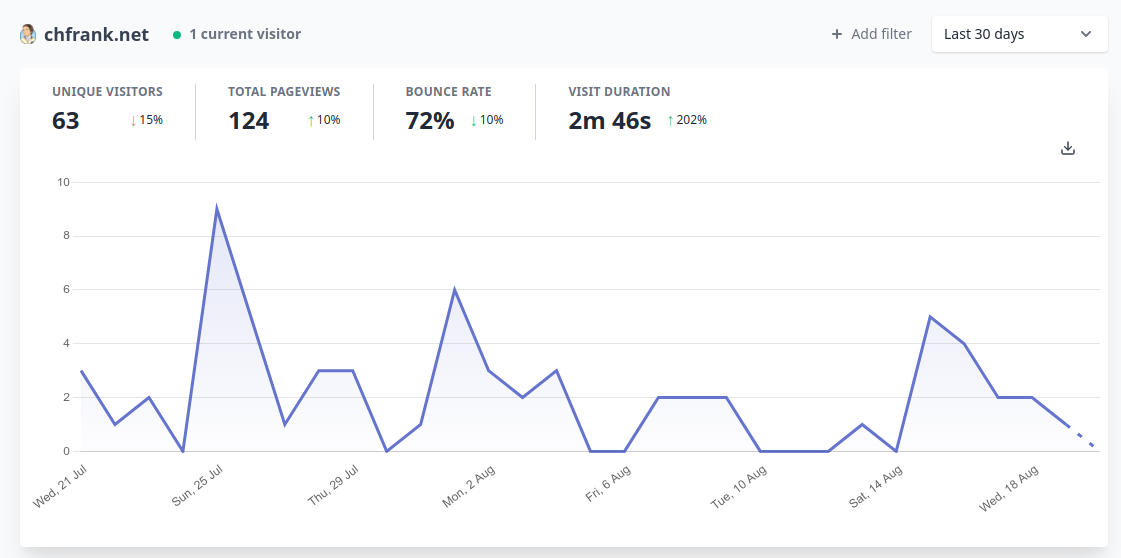
\includegraphics[width=\linewidth]{images/plausible.png}
\label{fig:plausible}
\end{figure}

\subsubsection{Yandex Metrica}

In case we're reluctant to send data to the US for processing but are at the same time not invested in the open source side of software, \href{https://metrica.yandex.com/}{Yandex Metrica} is another commercial option for web page analytics, covering more than 8 million sites, according to their web page.

Metrica is part of the Yandex family of tools; Yandex is headquartered in Moscow, Russia, and operates the biggest search engine there.

Yandex Metrica and Google Analytics are both operated by major search engine providers, which is not that surprising - in addition to crawling the web, these search engines need to perform a lot of analytics themselves to put the most relevant search results on the first page. It makes a lot of sense to expose these analytics in some form to the end users.

Optimizing our placement on the search engine result page is a wholly different topic that is out of scope for this paper.

\subsection{Toolstack - Advertising}

\subsubsection{Google Ads}

Now that we have identified the data sources for successful advertising campaigns and the tools to measure the success, we need to look at the platforms where we could place our campaigns. 

The biggest platform is \href{https://ads.google.com/home/}{Google Ads} and we can use it to run campaigns on Google's search engine result pages and affiliates.

Ad placement on Google is based on search keywords and Google's knowledge of the user's profile; Google operates a bidding website where we place bids for certain terms and demographics to get our particular ad shown. Ad placement and the underlying algorithm is a science unto itself; recently, Google has come under scrutiny from the regulators and, in one case, agreed to the ruling and the fine.\footnote{See \textit{Burgess, M. (2021)}: France Cracked Down on Google’s Ad Tech \cite{googleAds}}

To target the most appropriate users for an ad, Google needs to have accurate information on the user itself, and that's where third party data and data from third party cookies come in.

It's important to differentiate between ad placement, which is a paid-for service, and search engine result page placement, which can be improved through Search Engine Optimization (SEO) methods - even though both techniques are related to the Google search engine, they are not the same.

\subsubsection{Amazon Advertising}

The second biggest advertising platform is \href{https://advertising.amazon.com//}{Amazon Advertising}, a platform to place ads for our products on Amazon's pages and their affiliates.

The most significant difference to Google Ads is that Amazon Advertising already has all the relevant data from their users through the Amazon shopping web site. Amazon Advertising can operate almost entirely with its own first party data. It has user preferences, shopping history, and recent searches, all from its own data source and obtained with full consent from its users.

Amazon Advertising also operates as a demand-side platform with selected partners, to increase the reach of the ads placed, which would be a case of cooperation and the use of second party data.

With ads focused on the Amazon shopping experience and consent from their users obtained on sign-up, Amazon's advertising business is not that much affected by the current discussion about third-party data.

\subsubsection{Facebook Advertising}

Last but not least, we need to mention \href{https://www.facebook.com/business/ads}{Facebook Ads}, a platform to place ads on Facebook, Instagram, Messenger and the Audience Network.

Similar to Amazon, Facebook already has all the user profile data that it needs from its own platforms and has obtained consent during sign-up to share that data within its own family of businesses.\footnote{See \textit{WhatsApp (2021)}: What information does WhatsApp share with the Facebook Companies? \cite{whatsApp}}

Both companies, Amazon and Facebook, sit on a vast trove of invaluable first and second party data that they can freely use for their advertising business without needing to resort to third party data.

Knowing this, Facebook is currently running an extensive campaign at the moment to recruit new business customers for their personalized advertising offering.\footnote{See \textit{Facebook (2021)}: Dein Unternehmen ist es wert, entdeckt zu werden \cite{facebookAds}}

\subsection{Moving past cookies}

\subsubsection{Browser-based}

To continue with targeted advertising, even after the demise of the tracking cookie, new concepts and data sources are needed, some of which we will present and analyze in this paper with the goal of developing possible strategies for online marketing in the future.

A common thread of all the new approaches is the attempt to make targeted advertising work while at the same time maintaining the user's privacy; an umbrella term for these approaches is Privacy Preserving Advertising.\footnote{See \textit{Rescorla, E. (2021)}: The future of ads and privacy \cite{futureAds}}

The primary contender in the PPA space is \href{https://wicg.github.io/floc/}{Google FLoC}. The idea behind Google's federated learning of cohorts is actually quite simple. It aims to expose the users' general browsing interest without disclosing the browsing history, as it is the case today through the widespread use of third party cookies.

To achieve this, Google proposes an algorithm to assign cohort ids to individual browsers based on shared browsing habits. Then, instead of placing ads towards personally identifiable user profile data, ads would be placed against an anonymous cohort. 

The idea behind FLoC itself sounds quite reasonable; it is, however, under heavy fire from a privacy point of view.\footnote{See \textit{Rescorla, E. (2021)}: Privacy analysis of FLoC \cite{privacyFloc}} Among others, \href{https://www.eff.org/}{EFF}\footnote{Disclosure: I am a member and active supporter of EFF} has published a detailed analysis of FLoC's shortcomings in regards to privacy and why they believe that FLoC would be a terrible idea.\footnote{See \textit{Cyphers, B. (2021)}: Google’s FLoC Is a Terrible Idea \cite{terribleIdea}}

One of the biggest concerns is that by combining the FLoC data with browser fingerprinting, for example, super profiles could be created that would contain much more information than is available today. In summary, all currently available analyses question the actual ability of FLoC to maintain the user's privacy and foresee a much broader tracking of users and their profiles than currently through the use of third party cookies, should it come through.

It is worth noting that the issues with FLoC center around privacy, not the algorithm itself - federated learning is a well-established technique in the field of machine learning.\footnote{See \textit{Li, T. (2020)}: Federated Learning: Challenges, Methods, and Future Directions \cite{9084352}}

\subsubsection{Identity-based}

Similar to FLoC are several other approaches that implement some kind of advertising ID instead, which would attempt not to violate the user's privacy rights and still allow for targeted advertising. 

The most prominent approach was Apple's ID for Advertising, which does not seem to be going anywhere for the time being.\footnote{See \textit{Ray, O. (2020)}: What is IDFA and Why Apple Killed it \cite{cleanRoom}}

Google also has an Advertising ID that supports ad personalization based on preference.\footnote{See \textit{Google (2021)}: Advertising ID \cite{advertisingId}} Similar to Apple's ID, Google's Advertising ID offers an opt-out mechanism; if one opts out, only generic ads will be shown with much less relevance, and with a much lower chance of a sale for the company placing the ad.

An industry consortium is releasing an open-source ID standard, UID2.\footnote{See \textit{The Trade Desk (2021)}: Unified ID Solution 2.0 \cite{tradeDesk}} The basic premise is the same as for Google's or Apple's ID - the user is identified through a piece of personal information that is then encrypted and used as ID for the advertising profile. Unlike the approach from Apple and Google, however, the ID is not based on the device or the browser but would require an active login. Quite elegantly, this would solve all issues around consent and privacy. Still, it remains to be seen how many users will be logging in to an advertising network and share their preferences just to get better ads displayed.

Also, Microsoft is working together with the Harvard University on yet another standard\footnote{See \textit{Bird, S. (2020)}: Introducing the new differential privacy platform \cite{openDp}}, \href{https://opendp.org/}{OpenDP}, based on Differential Privacy.\footnote{See \textit{OpenDP (2020)}: What is Differential Privacy? \cite{diffPrivacy}} The conceptual idea behind differential privacy is quite interesting, but an analysis is out of scope for this paper.

\subsubsection{Data-based}

A completely different option would be to do away with third party data altogether and focus solely on second party data to augment one's own data. 

One way to achieve this could be through data clean rooms, where independent contract processors would anonymously combine first party data of two or more companies and return the aggregated results to all parties. Having independent data trustees that vouch for anonymity could make sure that such data processing would not run afoul of data protection regulations.\footnote{See \textit{Younger, M. (2019)}: The Three Hidden Technology Trends Behind Data Clean Rooms \cite{cleanRoom}}

Even though this approach sounds quite promising, such an independent infrastructure does not yet exist, and no supra-national body has stepped up to create; however, there are some nascent offerings, such as Google's \href{https://developers.google.com/ads-data-hub}{Ads Data Hub}.

\subsubsection{Content-based targeting}

Another quite interesting approach is to forfeit user-based targeting altogether and concentrate solely on the browsing context. In 2020, the public radio in The Netherlands did this and went from targeted advertising to contextual advertising; quite surprisingly, they saw their ad revenues grow.\footnote{See \textit{Edelman, G. (2020)}: Can Killing Cookies Save Journalism? \cite{killingCookies}} 

The system at \href{https://over.npo.nl/}{NPO} is a bidding system similar to Google Ads; however, ads are not placed based on a user profile, but on the current context, i.e., a web page that is shown or a TV show watched. As far as the documentation shows, there's never any personally identifiable information being collected or transmitted and thus no issue at all with violating the user's privacy.

Abandoning the user profile in favor of context feels a bit like going back in time, but it does eliminate all privacy woes.

\subsection{Legal Framework}

In the final chapter of this section, we need to have a brief look at the privacy laws and regulations that have come up in recent times. 

With privacy coming into focus more and more, legislation is being drafted all over the world to better protect the user's privacy, eliminate unauthorized data collection and fight surveillance capitalism.\footnote{See \textit{Zuboff, S. (2020)}: You Are Now Remotely Controlled \cite{surveillance}} 

There's quite a number of legal frameworks that begin to govern tracking and advertising, so here's a list of the most common ones with links to the respective legal texts:

\begin{itemize}
 \item \href{https://gdpr-info.eu/}{GDPR} (General Data Protection Regulation)
 \item \href{https://www.datenschutz-grundverordnung.eu/}{DS-GVO} (Datenschutzgrundverordnung)
 \item \href{https://dsgvo-gesetz.de/bdsg/}{BDSG} (Bundesdatenschutzgesetz)
 \item \href{https://dsgvo-gesetz.de/ttdsg/}{TTDSG} (Telekommunikations-Telemedien-Datenschutz-Gesetz (Entwurf ))
 \item \href{https://oag.ca.gov/privacy/ccpa}{CCPA} (California Consumer Privacy Act)
 \item \href{https://www.lgpdbrasil.com.br/}{LGPD} (Lei Geral de Proteção de Dados Pessoais)
 \item \href{https://popia.co.za/}{POPIA} (Protection of Personal Information Act)
 \item \href{https://ec.europa.eu/info/strategy/priorities-2019-2024/europe-fit-digital-age/digital-services-act-ensuring-safe-and-accountable-online-environment_en}{DSA} (Digital Services Act)
 \item \href{https://ec.europa.eu/info/strategy/priorities-2019-2024/europe-fit-digital-age/digital-markets-act-ensuring-fair-and-open-digital-markets_en}{DMA} (Digital Markets Act)
\end{itemize}

We cannot dive into the details on all these regulations; for the purpose of this paper, we will assume that the reader is familiar with the content of the most important ones for Europe and Germany, the GDPR/DS-GVO and the BDSG, and will from here on solely focus on their impact and interpretation.

Until here we've covered all fundamental aspects of tracking and targeting and introduced the most relevant tools and current developments. To continue developing strategies for online marketing beyond the end of the tracking cookie, it's time to bring in the experts.
